
\subsection{Punto \textbf{2b}}

\begin{itemize}
\item \emph{\textbf{Simular el mismo inversor del punto anterior pero con cargas de \num{4}, \num{8} y \num{16} inversores mínimos ($W_{N} = 0.23 \si[per-mode=symbol]{\micro\meter}$ y $W_{P} = 2 \cdot W_{N}$).}}
\end{itemize}

En la figura~\figref{fig:fig_inverter_minimum_schematic} puede verse el circuito diseñado para el inversor mínimo, y pueden verse los parámetros seleccionados para los transistores.




\begin{figure}[H] %htb
\begin{center}
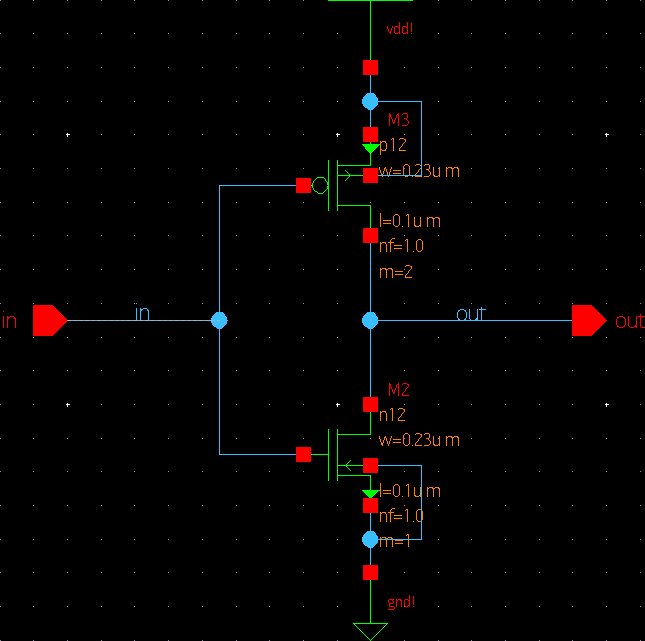
\includegraphics[width=0.85 \textwidth, angle=0]{./img/point2/TEST_LOGIC_GATES_Inverter_load_schematic}
\caption{\label{fig:fig_inverter_minimum_schematic}\footnotesize{Inversor \textbf{CMOS} mínimo diseñado (esquemático).}}
\end{center}
\end{figure}


\clearpage


En la figuras~\figref{fig:fig_inverter_4_min_load_schematic}~\figref{fig:fig_inverter_8_min_load_schematic}~y~\figref{fig:fig_inverter_16_min_load_schematic} pueden verse los circuito de los test bench armados para simular la respuesta del inversor con esas cargas.


\begin{figure}[H] %htb
\begin{center}
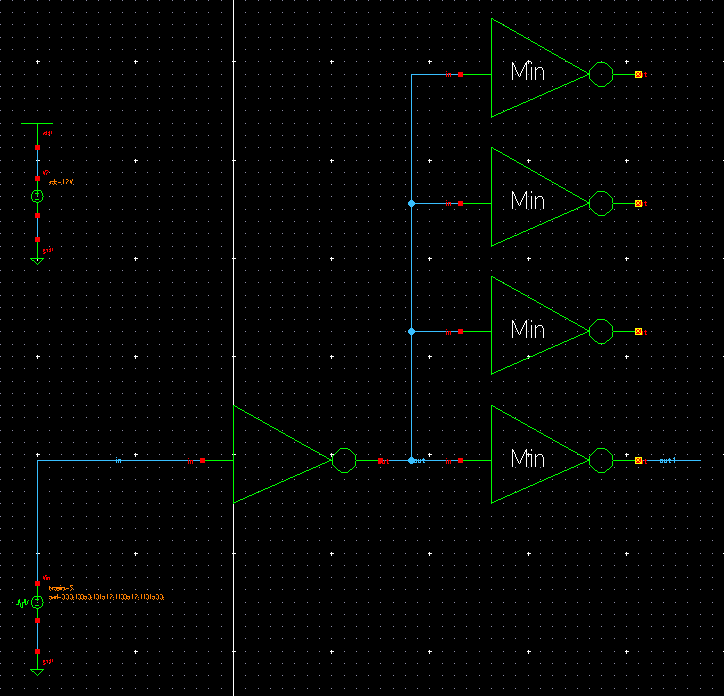
\includegraphics[width=0.8 \textwidth, angle=0]{./img/point2/TEST_LOGIC_GATES_tb_inverter_4_response_schematic}
\caption{\label{fig:fig_inverter_4_min_load_schematic}\footnotesize{Inversor \textbf{CMOS} cargado con 4 inversores mínimos, test bench diseñado (esquemático).}}
\end{center}
\end{figure}

\vfill
\clearpage

\begin{figure}[H] %htb
\begin{center}
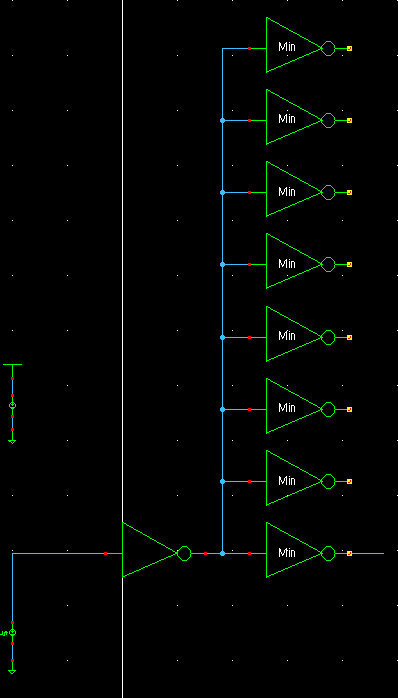
\includegraphics[width=0.4 \textwidth, angle=0]{./img/point2/TEST_LOGIC_GATES_tb_inverter_8_response_schematic}
\caption{\label{fig:fig_inverter_8_min_load_schematic}\footnotesize{Inversor \textbf{CMOS} cargado con 8 inversores mínimos, test bench diseñado (esquemático).}}
\end{center}
\end{figure}

\vfill
\clearpage

\begin{figure}[H] %htb
\begin{center}
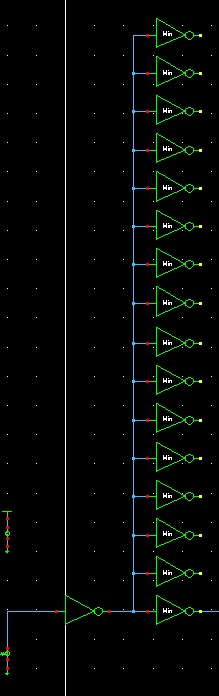
\includegraphics[width=0.2 \textwidth, angle=0]{./img/point2/TEST_LOGIC_GATES_tb_inverter_16_response_schematic}
\caption{\label{fig:fig_inverter_16_min_load_schematic}\footnotesize{Inversor \textbf{CMOS} cargado con 16 inversores mínimos, test bench diseñado (esquemático).}}
\end{center}
\end{figure}




En la figura~\figref{fig:fig_inverter_multiple_load_response} puede verse la respuesta obtenida con los circuitos de prueba de las figuras~figuras~\figref{fig:fig_inverter_4_min_load_schematic}~\figref{fig:fig_inverter_8_min_load_schematic}~y~\figref{fig:fig_inverter_16_min_load_schematic}.\\ 




En el cuadro~\tableref{table:delay_times}, se pueden ver resumidos los retardos obtenidos.



\begin{table}[H]  %%\centering

    \setlength\arrayrulewidth{1.5pt}
    \arrayrulecolor{white}
    \def\clinecolor{\hhline{|>{\arrayrulecolor{white}}-%
    >{\arrayrulecolor{white}}|-|-|-|-|}}
\resizebox{0.80 \textwidth}{!}{% 
       
\begin{tabularx}{1 \textwidth}%
    {|
    >{\columncolor{white} \centering\arraybackslash}m{0.2\textwidth}
     |
    >{\columncolor{white} \centering\arraybackslash}m{0.27\textwidth}
     |
    >{\columncolor{white} \centering\arraybackslash}m{0.27\textwidth}
     |
    >{\columncolor{white} \centering\arraybackslash}m{0.27\textwidth}
     |   
    }
    \rowcolor{HeadersColor} \cellcolor{white} \thead{}  & \thead{4 inversores min.} & \thead{8 inversores min.} & \thead{16 inversores min.} \\  
    \hhline{|-|-|-|-|}
    \rowcolor{gray!20} \cellcolor{gray!40} \textbf{Tiempo de retardo} & $7.5063 \si[per-mode=symbol]{\pico\second}$ & $11.2710 \si[per-mode=symbol]{\pico\second}$ & $21.5551 \si[per-mode=symbol]{\pico\second}$ \\
    \end{tabularx}}
	\caption{\footnotesize{Tiempos de retardo obtenidos para el inversor cargado con 4, 8 y 16 inversores mínimos.}}
	\label{table:delay_times}
\end{table}



Se puede apreciar que el retardo del inversor cargado con 4 inversores mínimos, coincide bastante bien con la respuesta al estar cargado con un inversor idéntico, que justamente tiene transistores con 4 veces el área de los transistores del inversor mínimo. El tiempo de retardo parece escalar con el área de los transistores, cosa que también se aprecia en las respuestas obtenidas con 4, 8 y 16 inversores mínimos.



\vfill
\clearpage





\begin{figure}[H] %htb
\begin{center}
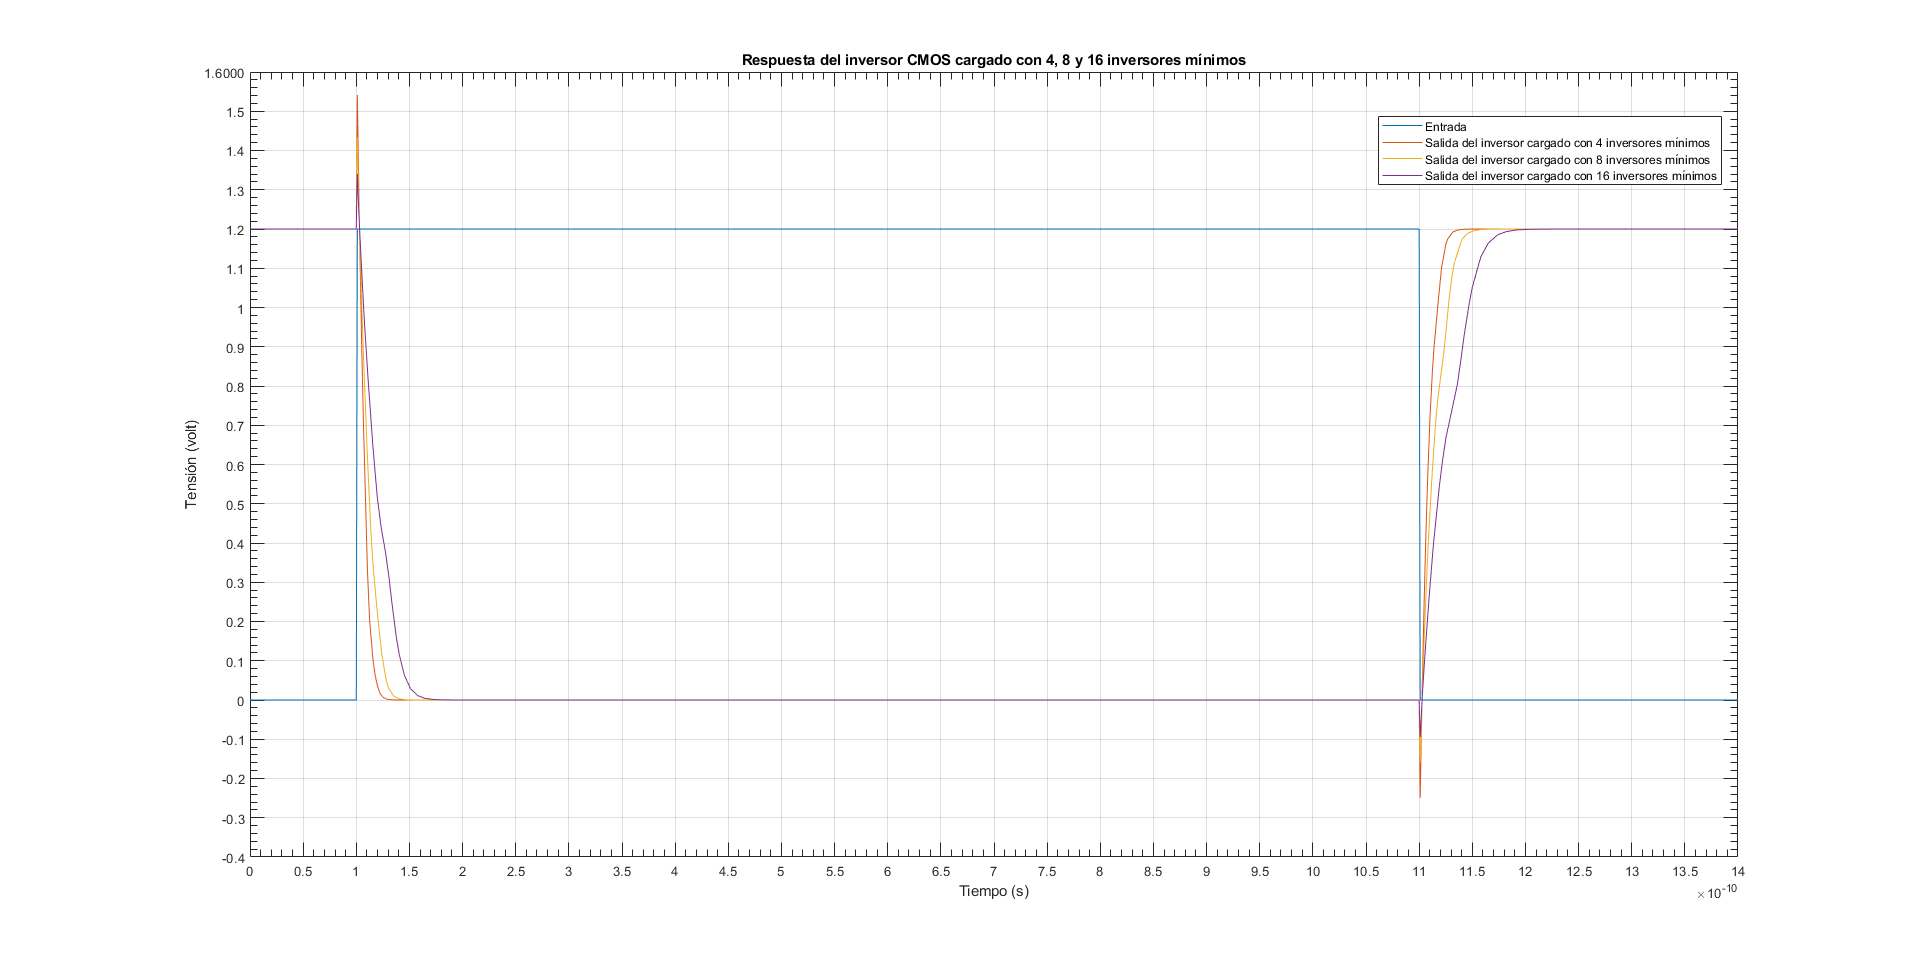
\includegraphics[width=0.92 \textheight, angle=90]{./img/point2/4_8_16_inverters_load_response}
\caption{\label{fig:fig_inverter_multiple_load_response}\footnotesize{Respuesta del inversor \textbf{CMOS} cargado con 4, 8 y 16 inversores mínimos.}}
\end{center}
\end{figure}




